\documentclass[a4paper, 14pt]{article}


\usepackage{cmap}
\usepackage[T2A]{fontenc}
\usepackage[utf8]{inputenc}
\usepackage[english,russian]{babel}
\usepackage{amsmath}
\usepackage{amsfonts}
\usepackage{amsmath,amsthm,amssymb}
\usepackage{color}
\usepackage{pgfplots}
\usepackage{tikz}
\pgfplotsset{compat=1.9}
\usepackage{graphicx}
\usepackage{float}
\usepackage{wrapfig}
\usepackage{bchart}




\begin{document}

	\renewcommand{\chaptername}{Лабораторная работа}
	\def\contentsname{Содержание}

	\begin{titlepage}
		\begin{center}
			\textsc{<<НАЦИОНАЛЬНЫЙ ИССЛЕДВАТЕЛЬСКИЙ УНИВЕРСИТЕТ ИТМО">\\[5mm]
			Факультет информационных технологий и программирования\\[2mm]
			Кафедра компьютерных технологий}

			\vfill

			\textbf{ОТЧЁТ ПО ЛАБОРАТОРНОЙ РАБОТЕ №2\\[3mm]
			Методы градиентной оптимизации\\[28mm]
			}
		\end{center}

		\hfill
		\begin{minipage}{.5\textwidth}
			Выполнили студенты:\\[2mm]
			Ефимов Сергей Алексеевич\\
			группа: М3237\\[2mm]
			Соколов Александр Андреевич\\
			группа: М3234\\[5mm]

			Проверил:\\[2mm]
			Свинцов Михаил Викторович
		\end{minipage}%
		\vfill
		\begin{center}
			г. Санкт-Петербург
		\end{center}
	\end{titlepage}


	\section*{Постановка задачи}
	Задача лаборатрной работы  -- научиться реализовывать алгоритмы градиентной оптимизации каждым из следуших способов:
	\begin{enumerate}
		\item Метод градиентного спуска
		\item Метод наискорейшего спуска
		\item Метод сопряженных градиентов
	\end{enumerate}
	Также необходимо оценить как меняется скорость сходимости, если для поиска величины шага использовать различные методы одномерного поиска.
	\section*{Ход работы}
	Фомализем поставленную задачу:
	Пусть мы имеем отображение из $f: \chi \subset \mathbb{R}^n \longrightarrow \mathbb{R}$, тогда $f$ - квадратичная функция. Необходимо реализовать алгоритмы минимизации данной функции, которые на выходе отдают $x^* = (x', y')$ - точка минимума, $f(x^*) = m$ - минимум функции
	Также мы будем испльзовать такие понятия как градиент $\nabla f(x)$ - вектор-столбец частных производных 1-ого порядка в этой точке, Матрица А - симметричная матрица коэфициентов при $x_i \cdot x_j$ , b — вектор-столбец при $x_i$ , $c \in \mathbb{R}$.	
		\subsection*{Оценка скорости сходимости}
		Давайте рассмотрим зависимость скорости сходмости алгоритма от метода поиска шага однмерной сходимости 
		
		Без ограничений общности возьмем функцию от двух переменных, у которой матрица А диагональная:
		\[
		f(x, y) = 5x^2 + 7y^2 - 8x + 9y + 10
		\]
		
		Минимум данной функции $\min f(x, y) = 3.908$ 
		Минимум достигается в точке $X(0.8, -0.643)$
		Точность для для каждого из методов была выбрана одинаковая($\epsilon = 10^{-5}$)
		
		\begin{bchart}[step=2, max=25]
        \bcbar[value=Dichotomy, color=yellow]{22}
            \medskip
        \bcbar[value=Golden Ratio, color=green]{18}
            \medskip
        \bcbar[value=Fibonacci, color=red]{18}
             \medskip
        \bcbar[value=Brent, color=blue]{18}
    \end{bchart} 
		\subsection*{Анализ функций}
		Возьмем три функции для анализа и приведем для каждого линии уровня
		\begin{itemize}
			\item $f(x, y) = x^2 + y^2$ \\
			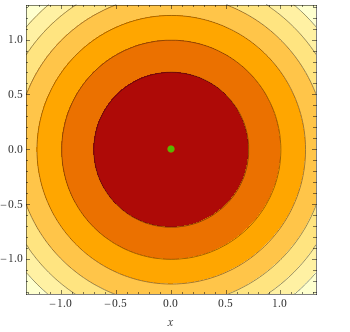
\includegraphics{img/1.png}
			\item $f(x, y) = 5x^2 + 7xy + 9y^2 + 11x + 12y + 14$ \\
			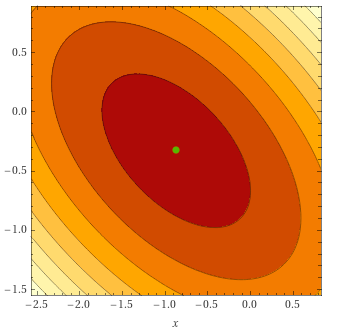
\includegraphics{img/2.png}
			\item $f(x, y) = 254x^2 + 506xy + 254y^2 + 50x + 130y - 111$ \\
			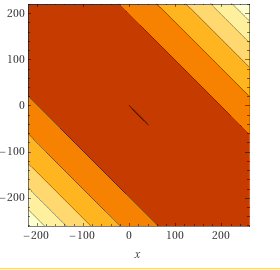
\includegraphics{img/3.png}
		\end{itemize}
		
		Приведем аналитическое реешние для данных функций и найдем минимум:\\
		

		\[1) f(x, y) = x^2 + y^2\]
		\[\min x^* = (0, 0), f(x^*) = 0\]
		\[2) f(x, y) = 5x^2 + 7xy + 9y^2 + 11x + 12y + 14\]
		\[f'_x = 10x + 7y + 11\]
		\[f'_y = 7x + 18y + 12\]
		\[\begin{cases}
		f'_x = 0\\
		f'_y = 0
		\end{cases}\]
		\[\begin{cases}
		10x + 7y + 11 = 0\\
		7x + 18y + 12 = 0
		\end{cases}\]
		\[\begin{cases}
		x^* = -\frac{114}{131}\\
		y^* = -\frac{43}{131}
		\end{cases}\]
		\[f''_{xx} \cdot f''_{yy} - f''_{xy} \cdot f''_{yx} = 10 \cdot 18 - 7 \cdot 7 > 0\]
		Откуда $\min x^* = (-\frac{114}{131}, -\frac{43}{131})$ 
		
		\[3) f(x, y) = 254x^2 + 506xy + 254y^2 + 50x + 130y - 111\]
		\[f'_x = 508x + 506y + 50\]
		\[f'_y = 506x + 508y + 130\]
		\[\begin{cases}
		f'_x = 0\\
		f'_y = 0
		\end{cases}\]
		\[\begin{cases}
		508x + 506y + 50 = 0\\
		506x + 508y + 130 = 0
		\end{cases}\]
		\[\begin{cases}
		x^* = \frac{3365}{169}\\
		y^* = -\frac{3393}{169}
		\end{cases}\]
		\[f''_{xx} \cdot f''_{yy} - f''_{xy} \cdot f''_{yx} = 508 \cdot 508 - 506 \cdot 506 > 0\]
		Откуда $\min x^* = (\frac{3365}{169}, -\frac{3393}{169})$ 
		
		\subsection*{Общий принцип выполнения методов}
		Пусть есть $f$- минимизуемая функция. Задается некое первое приближения решения $x^{(0)}$. На каждом шаге метода мы вычисляем следущее приближение
		\[x^k = \Phi(x^{k - 1}, x^{k-2}, ..., x^0)\]
		В нашем случае можно рассмотреть некое упрощение поиска следущего приближения как
		\[x^k = x^{k-1} + \alpha_{k-1} + p^{k-1}\]
		Где $\alpha_k$ - величина шага на $k$-той итерации, а $p^k$ - направление поиска  
		
		
		\subsection*{Метод градиентного спуска}
		Задается
		\begin{itemize}
			\item $\epsilon$ - заданная точность
			\item $\alpha$ - величина шага на каждой итерации 
			\item $x^0$- первое приближение
		\end{itemize}
		Изначально вычисляем $f(x^0)$. На каждой итерации будем вычислять $\nabla f(x^k)$, если найденное значение меньше  $\epsilon$, то метод завершается и ответом становится последнее найденное приблиение, пересчет на $k$-той итерации происходит следущм образом:
		\begin{itemize}
			\item $t = x^{k-1} - \alpha \nabla f(x^{k-1})$
			\item Пока $f(t) >= f(x^{k-1}) $ повторять предыдущий пункт с $\alpha = \frac{\alpha}{2}$
			\item $x^k = t, f(x^k) = f(t)$
		\end{itemize}
		
		\subsection*{Метод наискорейшего спуска}
		Задается
		\begin{itemize}
			\item $\epsilon$ - заданная точность
			\item $x^0$- первое приближение
		\end{itemize}
		Метод похож на предыдущий с одним отличием, $\alpha$ не задается константная, анаходится одним из методов одномерной оптимизации(например, методом заолотого сечения)
		
		\subsection*{Метод сопряженных градиентов}
		Задается
		\begin{itemize}
			\item $\epsilon$ - заданная точность
			\item $x^0$- первое приближение
			\item $p^0$- начальное направление поиска
		\end{itemize}
		$p^0$ находится как $-\nabla f(x^0)$. Пересчет происходит по следущим правилам:
		\[x^k = x^{k -1} + \alpha_{k-1}p^{k-1}\]
		\[p^k = -\nabla f(x^{k}) + \beta_{k - 1}p^{k - 1}\]
		где 
		\[\alpha_k = \frac{||\nabla f(x^{k})||^2}{\left\langle Ap^k, p^k\right\rangle}\]
		\[\beta_k = \frac{\Vert f(x^{k + 1})\Vert^2}{\Vert f(x^k)\Vert^2}\]
		
		\subsection*{Зависимость числа итераций}
		1) Автор условия лабораторной работы предлагает ввести отношение $T(n, k)$, где n -- размерность пространства, а k -- число обусловленности, давайте проведем несколько эксперементов
		
		\begin{tikzpicture}
		\begin{axis}[
		title = Метод градиентного спуска,
		xlabel = {$k$ число обусловленности $\cdot 10^3$},
		ylabel = {кол-во итераций$\cdot 10^4$},
		minor tick num = 2,
		xmin = 0,
		xmax = 2,
		ymax = 2,
		samples = 100,
		width = 420
		]
		\legend{
			n = 10,
			n= 100,
			n = 1000,
			n = 10000
		};
		\addplot[red] {x};
		\addplot[black] {x*1.01};
		\addplot[green] {x*1.015};
		\addplot[yellow] {x};
		\end{axis}
	\end{tikzpicture}
	
	\begin{tikzpicture}
		\begin{axis}[
		title = Метод наискорейшего спуска,
		xlabel = {$k$ число обусловленности $ \cdot 10^3$},
		ylabel = { кол-во итераций $\cdot 10^4$},
		minor tick num = 2,
		xmin = 0,
		xmax = 2,
		samples = 100,
		width = 420
		]
		\legend{
			n = 10,
			n= 100,
			n = 1000,
			n = 10000
		};
		\addplot[red] {x*0.75};
		\addplot[black] {x*0.75};
		\addplot[green] {x*0.75};
		\addplot[yellow] {x*0.78};
		\end{axis}
	\end{tikzpicture}
	
	\begin{tikzpicture}
		\begin{axis}[
		title = Метод сопряженных градиентов,
		xlabel = {$k$ число обусловленности $ \cdot 10^2$},
		ylabel = {кол-во итераций $\cdot 10^4$},
		xmin = 0,
		xmax=2,
		ymax=4,
		ymin=0,
		samples =300,
		width = 420
		]
		\legend{
			n = 10,
			n= 100,
			n = 1000,
			n = 10000
		};
		\addplot[yellow] {sqrt(x) * 0.1};
		\addplot[green] {sqrt(x) * 0.5};
		\addplot[red] {sqrt(x) * 1.1};
		\addplot[black] {sqrt(x) * 2};
		
		\end{axis}
	\end{tikzpicture}
		Исходя из графиков можно сделать вывод о том, что число обусловленности $k$ влияет на то, насколько может изменится значение фукнции при изменении аргумента
		
		\subsection*{Вывод}
		 Исходя из проделанной работы можно сделать вывод о том, что метод градиентного и наискорейшего спуска обладают линейной зависимостью числа итераций от числа обусловленности, так же стоит заметить, что они ведут себя примерно одинаково при одних и тех же входных данных. Размерность пространства не влияет на кол-во итераций 
		 
		 На методе сопряженных градиентов можем наюлдать другую картину, число итераций растет пропорцианально $\sqrt{k}$ от числа обусловленности, такую же тенденцию можно наблюдать в зависимсти от размерности
		 
			

		
		

  
\end{document}
